% ------------------------- MAIN TASK ---------------------------------
\section{Main task}
\subsection{Schematic proposal for limiting output current to 250mA} \label{ssec:num11}
{
	We were asked to design a proposed scheme to limit the output current to 250mA, to do this we decided to change the principle of the connections to create a current source using the LM317.	
	
	\begin{figure}[h]
		\centering
		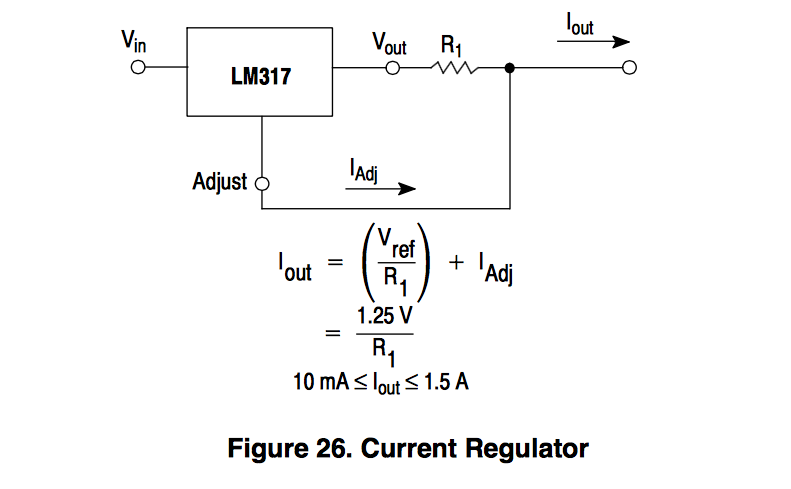
\includegraphics[width=0.7\linewidth]{../Figures/Partie2/SourceCourant}
		\caption{Current source with LM317}
		\source{Stackexchange "lm317-µa-constant-current-source-possibility"}
		\label{fig:sourcecourant}
	\end{figure}
	
	We use the reference voltage (\textbf{1.25V}) of the internal diode, so the output current depends on the resistance \textbf{R1} plus the leakage current of the diode.
	
	By adding and changing a load resistor in the circuit, the induced output current will vary, as will the voltage, but the current will not exceed : \\ $\frac{Vref}{R1}+I_{ADJ}$ \vspace{+6pt}
	
}

\newpage
\subsection{Plotting output tension depending on output current} \label{ssec:num12}
{
One of the unique features of the LM317 is its ability to automatically adjust its output voltage in response to changes in temperature. This is accomplished using a built-in temperature-sensing circuit that monitors the temperature of the LM317 and adjusts the output voltage accordingly.\vspace{+12pt}

When the temperature of the LM317 increases, the temperature-sensing circuit will cause the output voltage to decrease slightly. This helps to prevent the LM317 from overheating and ensures that it continues to operate within safe temperature limits. Similarly, when the temperature of the LM317 decreases, the temperature-sensing circuit will cause the output voltage to increase slightly. This helps to maintain a stable and consistent output voltage, even in changing temperature conditions.\vspace{+12pt}

Overall, the LM317's ability to regulate according to temperature makes it a versatile and reliable choice for applications that require a constant output voltage, such as in power supply circuits and battery chargers. \vspace{+12pt}

We will observe this characteristic through our following measurements.

\subsubsection{List of all the instruments}

\begin{tabular}{l | l | l}
	Instrument & Designator & Reference \\ 
	\hline\hline & & \vspace{-8pt}\\ 
	Oscilloscope & P1 & ES.SLO2.05.01.08 \\
	Current probe & P2 & ES.SLO1.00.06.04 \\
	DC power supply & G1 & ES.SLO2.00.00.31 \\
	Electronic load & G2 & ES.SLO2.00.02.60 \\
	Waveform generator & G3 & ES.SLO2.00.00.138 
\end{tabular}

\clearpage

\subsubsection{Measurement schematic}

}

\newpage
\subsection{Oscillogram of the output current depending on the output tension} \label{ssec:num13}
{
	
\subsubsection{Measurement schematic}
\begin{figure}[h]
	\centering
	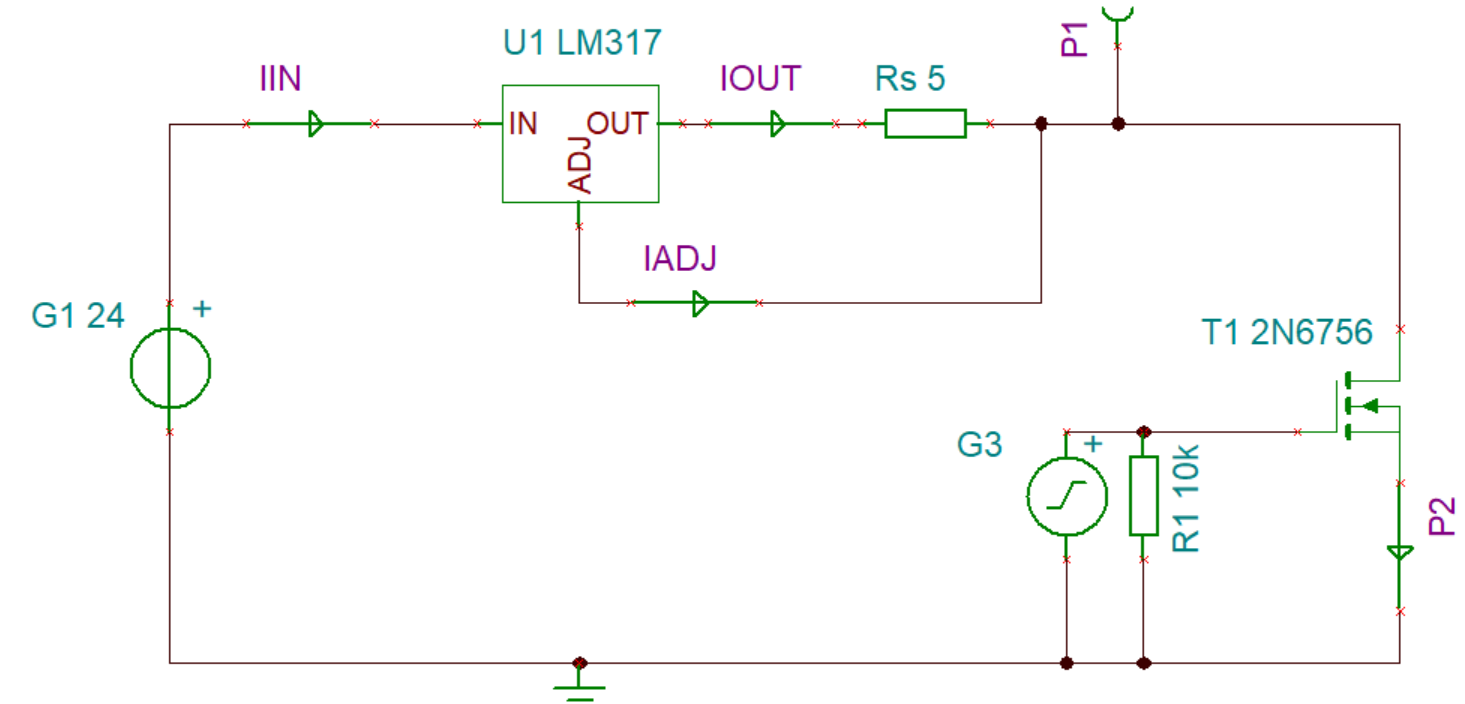
\includegraphics[width=0.8\linewidth]{../../schemaMesurePulses}
	\caption{Measurement schematic}
	\label{fig:schemamesurepulses}
	\source{Authors}
\end{figure}


}
\clearpage

\subsection{Dissipated power calculation} \label{ssec:num14}
{}
\subsection{Estimation of the junction's temperature without cooling} \label{ssec:num15}
{}
\subsection{Short-circuited output - dissipated power calculation} \label{ssec:num16}
{}

\section{Conclusion}
{}

\clearpage